\documentclass[aspectratio=169]{beamer}

% Default packages
\usepackage[T1]{fontenc}
\usepackage[english]{babel}
\usepackage{pgfplots}
\pgfplotsset{compat=newest}
\usepackage{booktabs}
\usepackage{siunitx}
\usepackage{amsmath}

% Font selection
% Latin Modern
\usepackage{lmodern}
% Verdana font type
%\usepackage{verdana}
% Helvetica
%\usepackage{helvet}
% Times (text and math)
%\usepackage{newtx, newtxmath}
% Nice font combination
%\usepackage{mathptmx} % math
%\usepackage{sourcesanspro} % sans-serif
\usepackage{charter} % serif

%Avoid shaded in RMarkdown
\usepackage{color}
\usepackage{fancyvrb}
\newcommand{\VerbBar}{|}
\newcommand{\VERB}{\Verb[commandchars=\\\{\}]}
\DefineVerbatimEnvironment{Highlighting}{Verbatim}{commandchars=\\\{\}}
% Add ',fontsize=\small' for more characters per line
\usepackage{framed}
\definecolor{shadecolor}{RGB}{248,248,248}
\newenvironment{Shaded}{\begin{snugshade}}{\end{snugshade}}
\newcommand{\AlertTok}[1]{\textcolor[rgb]{0.94,0.16,0.16}{#1}}
\newcommand{\AnnotationTok}[1]{\textcolor[rgb]{0.56,0.35,0.01}{\textbf{\textit{#1}}}}
\newcommand{\AttributeTok}[1]{\textcolor[rgb]{0.77,0.63,0.00}{#1}}
\newcommand{\BaseNTok}[1]{\textcolor[rgb]{0.00,0.00,0.81}{#1}}
\newcommand{\BuiltInTok}[1]{#1}
\newcommand{\CharTok}[1]{\textcolor[rgb]{0.31,0.60,0.02}{#1}}
\newcommand{\CommentTok}[1]{\textcolor[rgb]{0.56,0.35,0.01}{\textit{#1}}}
\newcommand{\CommentVarTok}[1]{\textcolor[rgb]{0.56,0.35,0.01}{\textbf{\textit{#1}}}}
\newcommand{\ConstantTok}[1]{\textcolor[rgb]{0.00,0.00,0.00}{#1}}
\newcommand{\ControlFlowTok}[1]{\textcolor[rgb]{0.13,0.29,0.53}{\textbf{#1}}}
\newcommand{\DataTypeTok}[1]{\textcolor[rgb]{0.13,0.29,0.53}{#1}}
\newcommand{\DecValTok}[1]{\textcolor[rgb]{0.00,0.00,0.81}{#1}}
\newcommand{\DocumentationTok}[1]{\textcolor[rgb]{0.56,0.35,0.01}{\textbf{\textit{#1}}}}
\newcommand{\ErrorTok}[1]{\textcolor[rgb]{0.64,0.00,0.00}{\textbf{#1}}}
\newcommand{\ExtensionTok}[1]{#1}
\newcommand{\FloatTok}[1]{\textcolor[rgb]{0.00,0.00,0.81}{#1}}
\newcommand{\FunctionTok}[1]{\textcolor[rgb]{0.00,0.00,0.00}{#1}}
\newcommand{\ImportTok}[1]{#1}
\newcommand{\InformationTok}[1]{\textcolor[rgb]{0.56,0.35,0.01}{\textbf{\textit{#1}}}}
\newcommand{\KeywordTok}[1]{\textcolor[rgb]{0.13,0.29,0.53}{\textbf{#1}}}
\newcommand{\NormalTok}[1]{#1}
\newcommand{\OperatorTok}[1]{\textcolor[rgb]{0.81,0.36,0.00}{\textbf{#1}}}
\newcommand{\OtherTok}[1]{\textcolor[rgb]{0.56,0.35,0.01}{#1}}
\newcommand{\PreprocessorTok}[1]{\textcolor[rgb]{0.56,0.35,0.01}{\textit{#1}}}
\newcommand{\RegionMarkerTok}[1]{#1}
\newcommand{\SpecialCharTok}[1]{\textcolor[rgb]{0.00,0.00,0.00}{#1}}
\newcommand{\SpecialStringTok}[1]{\textcolor[rgb]{0.31,0.60,0.02}{#1}}
\newcommand{\StringTok}[1]{\textcolor[rgb]{0.31,0.60,0.02}{#1}}
\newcommand{\VariableTok}[1]{\textcolor[rgb]{0.00,0.00,0.00}{#1}}
\newcommand{\VerbatimStringTok}[1]{\textcolor[rgb]{0.31,0.60,0.02}{#1}}
\newcommand{\WarningTok}[1]{\textcolor[rgb]{0.56,0.35,0.01}{\textbf{\textit{#1}}}}



% Use DTU theme, see below for options
\usetheme[department=compute]{DTU}

\title[Automated and Early Detection of Disease Outbreaks]{Models}
\author{Kasper Schou Telkamp}
\institute{Section for Dynamical Systems}
\date{2023-02-09}
	
\newcommand{\tabitem}{{\color{dtured}$\bullet$} }

\begin{document}


\frame{
	\maketitle
}

\frame{
	\frametitle{Outline}
	\tableofcontents
}

\hypertarget{data-exploration}{%
\section{Data exploration}\label{data-exploration}}

\hypertarget{vtec-stec}{%
\subsection{VTEC / STEC}\label{vtec-stec}}

\begin{frame}{VTEC / STEC}
\tiny

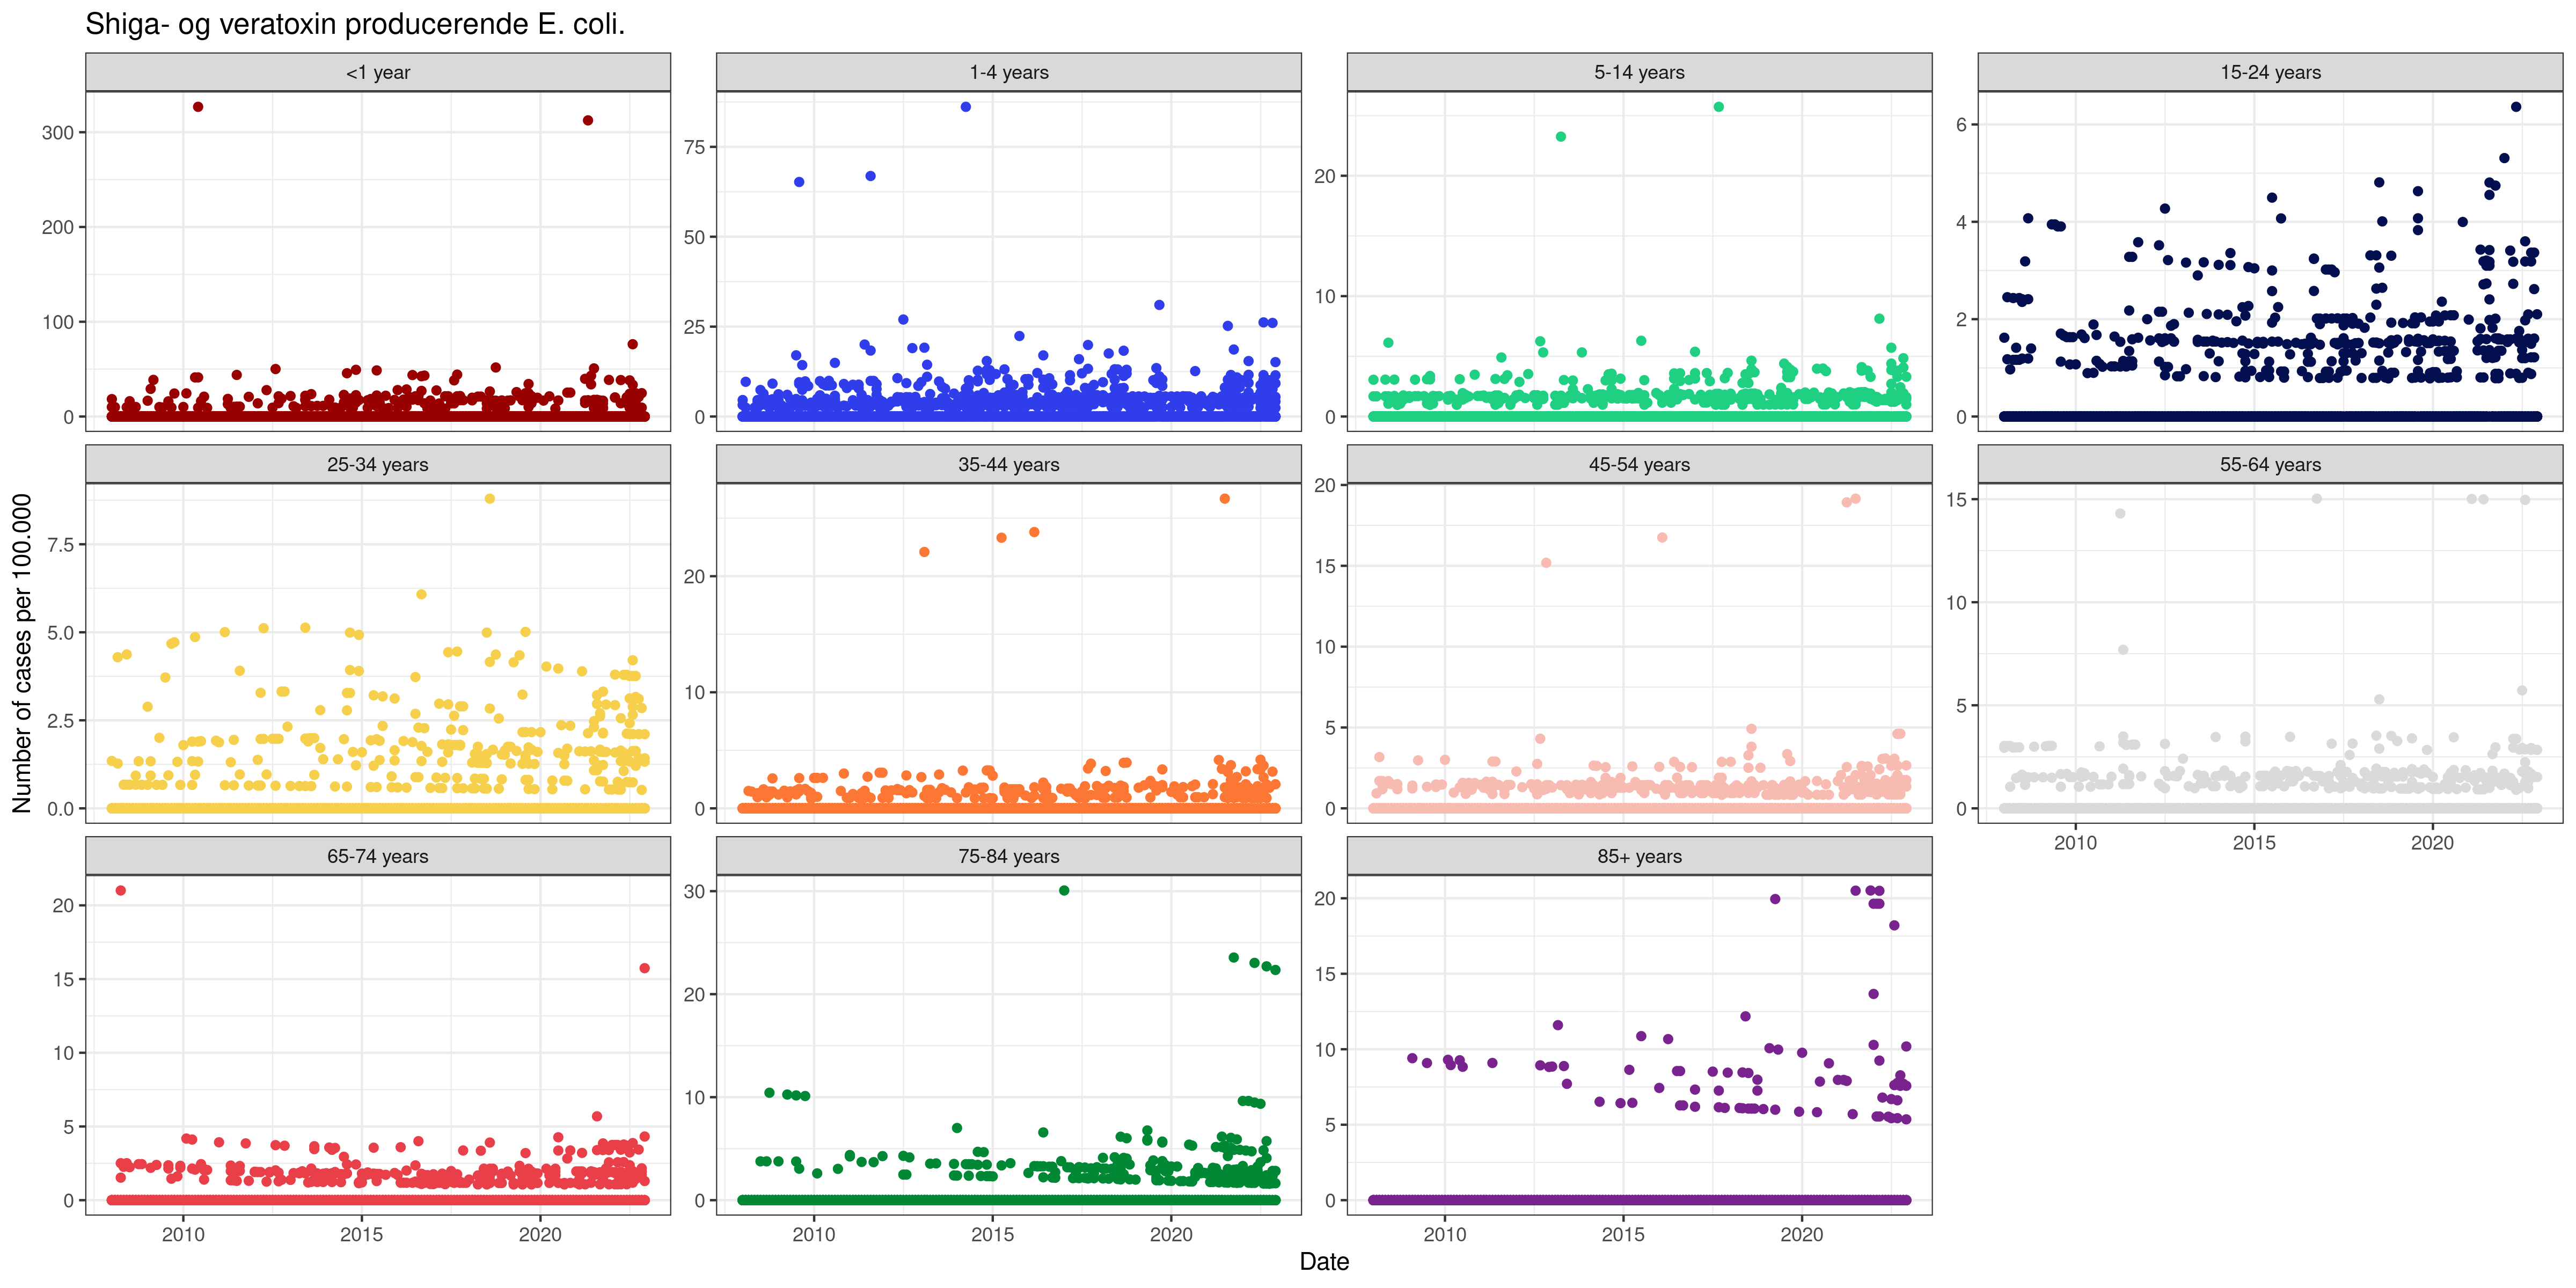
\includegraphics[width=1\linewidth]{../figures/ShigaogveratoxinproducerendeEcolixAgeGroup}

\normalsize
\end{frame}

\hypertarget{model-formulation}{%
\section{Model formulation}\label{model-formulation}}

\hypertarget{poisson-lognormal}{%
\subsection{Poisson-Lognormal}\label{poisson-lognormal}}

\begin{frame}{Poisson-Lognormal}
\begin{subequations}
  \begin{alignat}{2}
    Y_{i} &\sim \mathrm{Pois} \big( \lambda \exp(u_{i}) \big) \label{eq:pois_ln0} \\ 
    u_i &\sim \mathrm{N}(0,\sigma^2) \label{eq:pois_ln1}
  \end{alignat}
\end{subequations}
\end{frame}

\begin{frame}{Implementation - Test}
\protect\hypertarget{implementation---test}{}
\end{frame}

\begin{frame}[fragile]{Implementation - Objective function in C++}
\protect\hypertarget{implementation---objective-function-in-c}{}
\tiny

\begin{Shaded}
\begin{Highlighting}[]
\PreprocessorTok{\#include }\ImportTok{\textless{}TMB.hpp\textgreater{}}\PreprocessorTok{              }\CommentTok{// Links in the TMB libraries}

\KeywordTok{template}\OperatorTok{\textless{}}\KeywordTok{class}\NormalTok{ Type}\OperatorTok{\textgreater{}}
\NormalTok{Type objective\_function}\OperatorTok{\textless{}}\NormalTok{Type}\OperatorTok{\textgreater{}::}\KeywordTok{operator}\OperatorTok{()} \OperatorTok{()}
\OperatorTok{\{}
\NormalTok{  DATA\_VECTOR}\OperatorTok{(}\NormalTok{y}\OperatorTok{);}                       \CommentTok{// Data vector transmitted from R}
\NormalTok{  DATA\_FACTOR}\OperatorTok{(}\NormalTok{ageGroup}\OperatorTok{);}        \CommentTok{// Data factor transmitted from R}

\NormalTok{  PARAMETER\_VECTOR}\OperatorTok{(}\NormalTok{u}\OperatorTok{);}              \CommentTok{// Random effects}
   
  \CommentTok{// Parameters}
\NormalTok{  PARAMETER\_VECTOR}\OperatorTok{(}\NormalTok{lambda}\OperatorTok{);}       \CommentTok{// Parameter value transmitted from R}
\NormalTok{  PARAMETER}\OperatorTok{(}\NormalTok{log\_sigma\_u}\OperatorTok{);}               \CommentTok{// Parameter value transmitted from R}
  
\NormalTok{  Type sigma\_u }\OperatorTok{=}\NormalTok{ exp}\OperatorTok{(}\NormalTok{log\_sigma\_u}\OperatorTok{);}

  \DataTypeTok{int}\NormalTok{ nobs }\OperatorTok{=}\NormalTok{ y}\OperatorTok{.}\NormalTok{size}\OperatorTok{();}
\NormalTok{  Type mean\_ran }\OperatorTok{=}\NormalTok{ Type}\OperatorTok{(}\DecValTok{0}\OperatorTok{);}
  
  \DataTypeTok{int}\NormalTok{ j}\OperatorTok{;}

\NormalTok{  Type f }\OperatorTok{=} \DecValTok{0}\OperatorTok{;}               \CommentTok{// Declare the "objective function" (neg. log. likelihood)}
  \ControlFlowTok{for}\OperatorTok{(}\DataTypeTok{int}\NormalTok{ i}\OperatorTok{=}\DecValTok{0}\OperatorTok{;}\NormalTok{ i }\OperatorTok{\textless{}}\NormalTok{ nobs}\OperatorTok{;}\NormalTok{ i}\OperatorTok{++)\{}
\NormalTok{    f }\OperatorTok{{-}=}\NormalTok{ dnorm}\OperatorTok{(}\NormalTok{u}\OperatorTok{[}\NormalTok{i}\OperatorTok{],}\NormalTok{mean\_ran}\OperatorTok{,}\NormalTok{sigma\_u}\OperatorTok{,}\KeywordTok{true}\OperatorTok{);}
\NormalTok{    j }\OperatorTok{=}\NormalTok{ ageGroup}\OperatorTok{[}\NormalTok{i}\OperatorTok{];}
\NormalTok{    f }\OperatorTok{{-}=}\NormalTok{ dpois}\OperatorTok{(}\NormalTok{y}\OperatorTok{[}\NormalTok{i}\OperatorTok{],}\NormalTok{lambda}\OperatorTok{[}\NormalTok{j}\OperatorTok{]*}\NormalTok{exp}\OperatorTok{(}\NormalTok{u}\OperatorTok{[}\NormalTok{i}\OperatorTok{]),}\KeywordTok{true}\OperatorTok{);}
  \OperatorTok{\}}
  
  \ControlFlowTok{return}\NormalTok{ f}\OperatorTok{;}
\OperatorTok{\}}
\end{Highlighting}
\end{Shaded}

\normalsize
\end{frame}

\begin{frame}[fragile]{Implementation - Call from R}
\protect\hypertarget{implementation---call-from-r}{}
\tiny

\begin{Shaded}
\begin{Highlighting}[]
\CommentTok{\# Import libraries}
\FunctionTok{library}\NormalTok{(readr)}
\FunctionTok{library}\NormalTok{(dplyr)}
\FunctionTok{library}\NormalTok{(TMB)}

\CommentTok{\# Import the data}
\NormalTok{dat }\OtherTok{\textless{}{-}} \FunctionTok{read\_rds}\NormalTok{(}\AttributeTok{file =} \StringTok{"../../data/processed/dat.rds"}\NormalTok{)}

\CommentTok{\# Only consider some of the data}
\NormalTok{y }\OtherTok{\textless{}{-}}\NormalTok{ dat }\SpecialCharTok{\%\textgreater{}\%}
  \FunctionTok{filter}\NormalTok{(caseDef }\SpecialCharTok{==} \StringTok{"Shiga{-} og veratoxin producerende E. coli."}\NormalTok{) }\SpecialCharTok{\%\textgreater{}\%}
  \FunctionTok{group\_by}\NormalTok{(Date, ageGroup) }\SpecialCharTok{\%\textgreater{}\%}
  \FunctionTok{summarize}\NormalTok{(}\AttributeTok{y =} \FunctionTok{sum}\NormalTok{(cases))}

\FunctionTok{compile}\NormalTok{(}\AttributeTok{file =} \StringTok{"PoissonLognormal.cpp"}\NormalTok{)  }\CommentTok{\# Compile the C++ file}
\FunctionTok{dyn.load}\NormalTok{(}\FunctionTok{dynlib}\NormalTok{(}\StringTok{"PoissonLognormal"}\NormalTok{))    }\CommentTok{\# Dynamically link the C++ code}

\CommentTok{\# Function and derivative}
\NormalTok{f }\OtherTok{\textless{}{-}} \FunctionTok{MakeADFun}\NormalTok{(}
  \AttributeTok{data =} \FunctionTok{list}\NormalTok{(}\AttributeTok{y =}\NormalTok{ y}\SpecialCharTok{$}\NormalTok{y, }\AttributeTok{ageGroup =}\NormalTok{ y}\SpecialCharTok{$}\NormalTok{ageGroup),}
  \AttributeTok{parameters =} \FunctionTok{list}\NormalTok{(}\AttributeTok{u =} \FunctionTok{rep}\NormalTok{(}\DecValTok{1}\NormalTok{, }\FunctionTok{length}\NormalTok{(y}\SpecialCharTok{$}\NormalTok{y)),}
                    \AttributeTok{lambda =} \FunctionTok{rep}\NormalTok{(}\DecValTok{1}\NormalTok{, }\FunctionTok{nlevels}\NormalTok{(y}\SpecialCharTok{$}\NormalTok{ageGroup)),}
                    \AttributeTok{log\_sigma\_u =} \FunctionTok{log}\NormalTok{(}\DecValTok{1}\NormalTok{)),}
  \AttributeTok{random =} \StringTok{"u"}\NormalTok{,}
  \AttributeTok{DLL =} \StringTok{"PoissonLognormal"}
\NormalTok{)}
\end{Highlighting}
\end{Shaded}

\normalsize
\end{frame}

\hypertarget{poisson-gamma}{%
\subsection{Poisson-Gamma}\label{poisson-gamma}}

\begin{frame}{Poisson-Gamma}
\begin{subequations}
  \begin{alignat}{2}
    Y_{i} &\sim \mathrm{Pois} (\lambda u_{i}) \label{eq:pois_g0} \\ 
    u_i &\sim \mathrm{G}(1,\phi) \label{eq:pois_g1}
  \end{alignat}
\end{subequations}
\end{frame}


\end{document}
